\section{The Gap Left by Raw Retrieval}
\label{sec:problem}

\paragraph{Evidence-set retrieval.} A user's history is a sequence $H=(r_1,\dots,r_n)$. Each round contains a user turn, the following assistant turn, their attached images, and the session date. For a question $q$, let $G(q)\subseteq H$ be the evidence rounds and $S(q)\subseteq H$ the rounds retrieved for the reader. We measure whether retrieval finds all the annotated evidence with full-set recall,
\begin{equation}
\fsr(q)=\mathbf{1}\left[\,G(q)\subseteq S(q)\,\right],
\label{eq:fsr}
\end{equation}
and report the number of opened rounds $|S(q)|$ alongside it. Full-set recall is the per-question form of the all-recall measure used in multi-hop retrieval~\citep{gutierrez2024hipporag}: it checks whether the reader has every annotated item needed for a count or comparison.

\paragraph{Raw retrieval on text memory.} On LoCoMo and LongMemEval-S, cosine retrieval comes within one accuracy point of reading the full history, and the paired intervals include zero (Figure~\ref{fig:rag_motivation}; Appendix~\ref{app:text}). A retrieved subset is therefore sufficient on these text-memory tasks.

\paragraph{Incomplete evidence in multimodal memory.} Image-dependent questions expose a gap in retrieval coverage. Removing visual information sharply reduces accuracy on MemEye and VisualMem but barely changes it on Mem-Gallery, a text-dominant benchmark outside our scope (Figure~\ref{fig:setsize}a). On the image-dependent benchmarks, much of the evidence ranks low by embedding similarity: 11 to 14\% of the gold rounds on MemEye, MemLens, and CamRoll and 55\% on VisualMem lie outside the 40 rounds most similar to the question, where RAG@40 cannot open them (Figure~\ref{fig:setsize}b). Missing evidence is costly. With the lightweight reader, the accuracy of RAG@40 is 15 to 30 points lower on the questions for which its rounds miss part of the evidence than on the others (Figure~\ref{fig:setsize}c). Larger evidence sets are harder to complete: top-40 retrieval recovers only 30\% of the MemEye sets with six or more rounds (Figure~\ref{fig:setsize}d). These findings motivate selecting evidence with access to the wider history, including the context needed to resolve references across rounds.

\begin{figure*}[t]
\centering
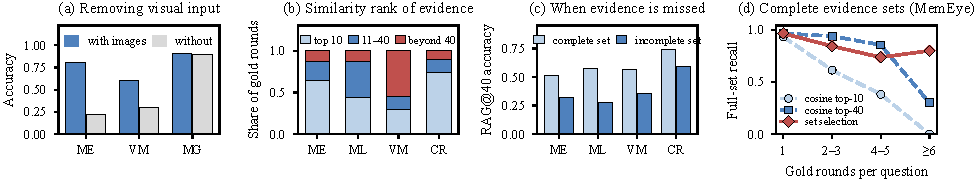
\includegraphics[width=\textwidth]{figures_polished/problem.pdf}
\caption{\textbf{Why similarity retrieval falls short on image evidence.} (a)~Accuracy with and without visual input. (b)~Gold evidence rounds by their embedding-similarity rank for the question. (c)~Lightweight-reader accuracy of RAG@40 on questions for which its 40 rounds contain all the evidence or miss part of it. (d)~Full-set recall on MemEye by evidence-set size. ME, ML, VM, CR, and MG denote MemEye, MemLens, VisualMem, CamRoll, and Mem-Gallery; reader and input conditions are given in Appendix~\ref{app:text}.}
\label{fig:setsize}
\end{figure*}
